\section{Overall Description}

\subsection{Product perspective}
 %Describes the environment of the system

\subsubsection{Description}
The SMSEncryption application is a new product that can accommodate the encryption/decryption of text to be sent via SMS, or any other text communcations service, such as Whatsapp, that can make use of more modern wireless data communication technologies - if it is available. Message text can be manipulated via any text manipulation application, such as the default Android/iOS keyboard, capable of using the basic GSM character set , that will be used by our application. Any third party keyboard applications such as SwiftKey can also be used.
\vspace{12pt}\\
The GSM character set contains a limited amount of characters, which will, in turn, limit the encryption methods we can make use of, as many encryption algorithms greatly increase both the size of the message, and the number of different characters used. Making use of these encryption algorithms that generate large amounts of characters will be infeasible, as sending a large amount of text via SMS will be expensive - as users generally pay a fixed amount per 160 characters.
\subsubsection{System interfaces}

\subsubsection{User interfaces}
 The user interface is what will allow the user to type a message, encrypt it, copy the ciphertext, and paste it into the application that will send the message. On the receiving end, the message received will be copied, and pasted into the SMSEncryption application, which will be used to decrypt the received message. This ensures integrity of the message, as only users of the application will be able to encrypt/decrypt the message if they have synchronized each other as contacts within the application.
\subsubsection{Hardware interfaces}
The software will run on a mobile device that allows user interaction and text manipulation.
\subsubsection{Software interface}
The software interface will make use of operating system features, such as the 'clipboard' on the device to facilitate 'copying' and 'pasting' of texts or ciphertexts.
\subsubsection{Memory}
The device needs minimal storage space, for the application, and the database it creates on the device, uses approximately 2mb.
\subsubsection{Operations}
\begin{itemize}
\item User-initiated operations:
\begin{itemize}
\item Create user account
\item Edit user account
\item Add contact
\item Edit contact
\item Remove contact
\item Enter message
\item Encrypt message
\item Decrypt message
\item Synchronise contact
\end{itemize}
\end{itemize}


%Note:
%Required : Functionality must be provided if service is provided
%Extends : Extended functionality which can be provided, but not always.
\subsubsection{Use Cases}
SMSEncryption Use Case Diagram

\begin{center}
 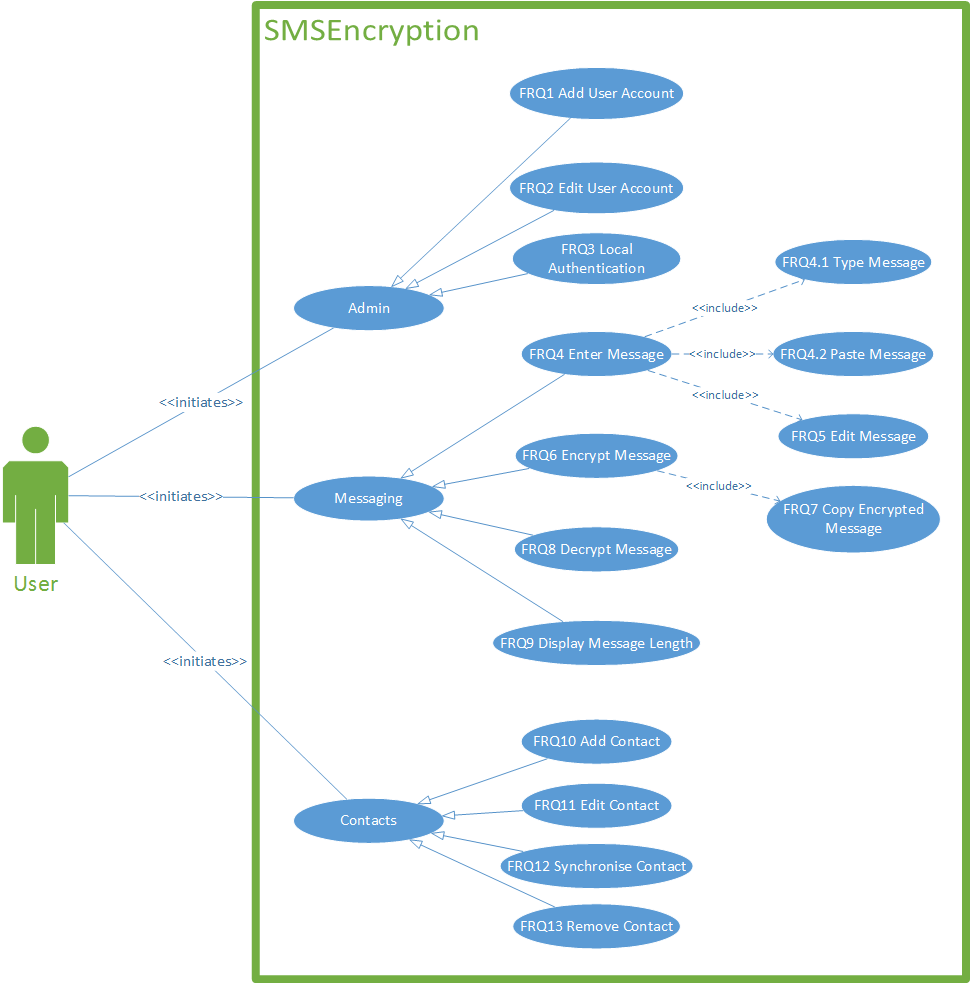
\includegraphics[width=13cm]{diagrams/UseCaseDiagrams/UsecaseV5.png}
\end{center}

\subsubsection{State Diagram}
SMSEncryption State Diagram

\begin{center}
 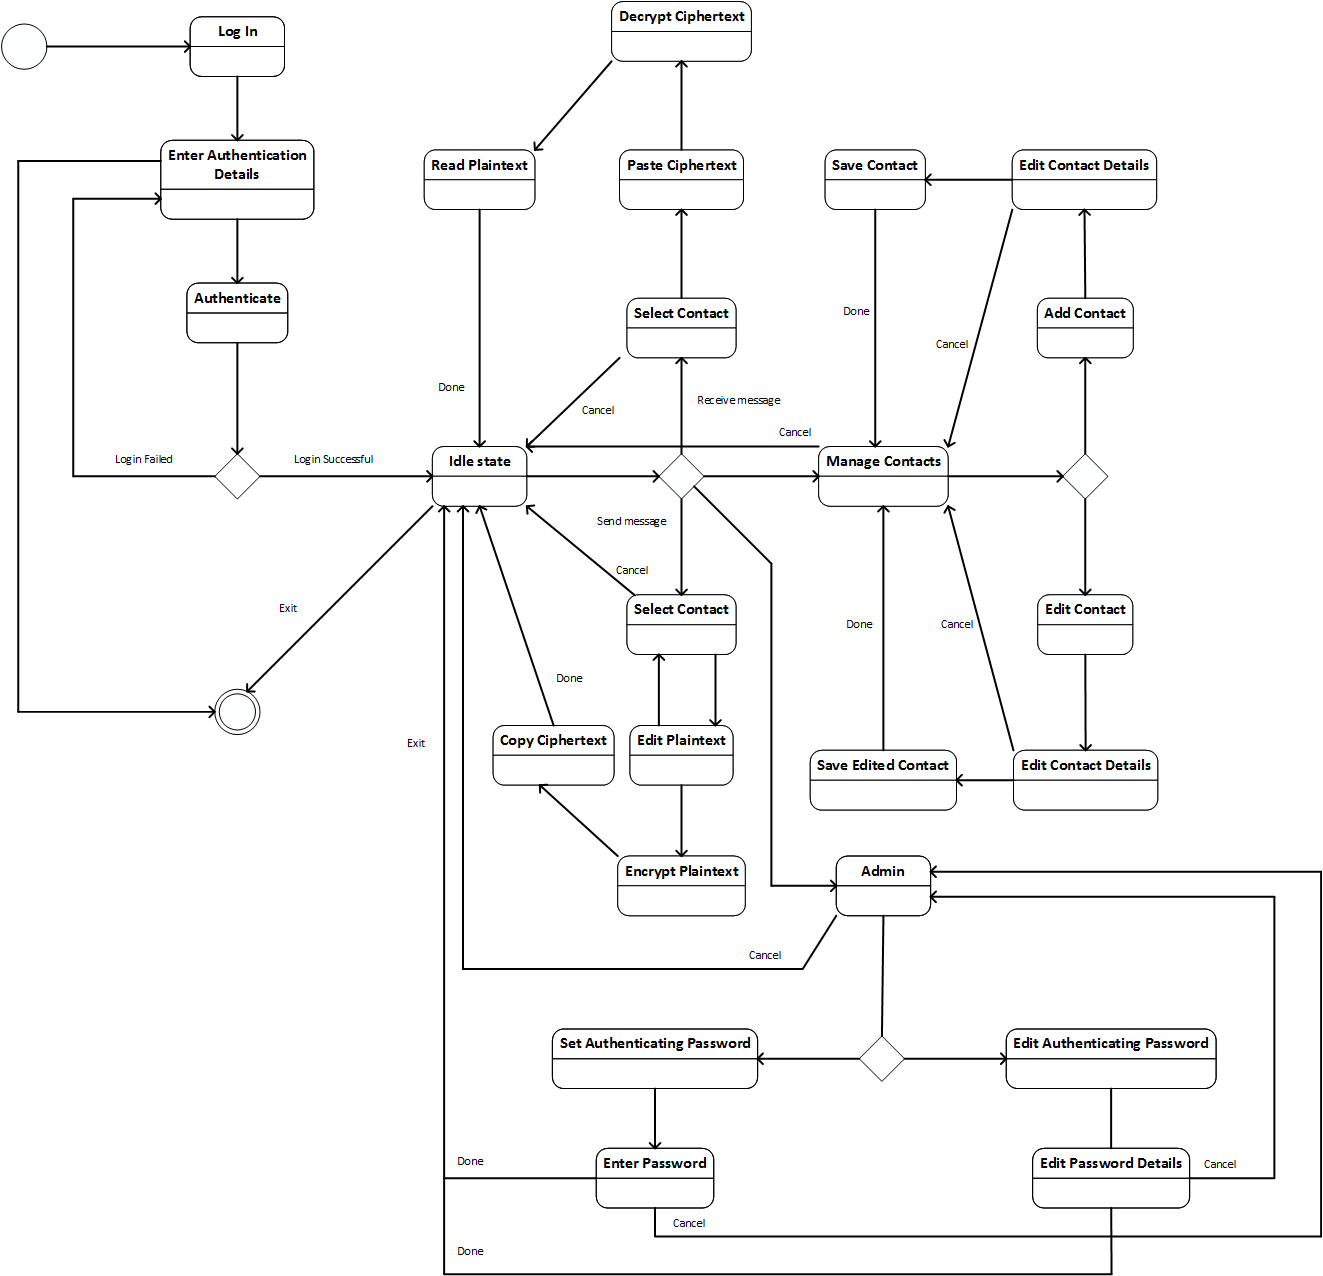
\includegraphics[width=13cm]{diagrams/StateDiagrams/SMSEncryptionStateMachine.png}
\end{center}


\subsection{Product functions}
The application is divided into 3 core functionalities: Admin, Messaging, and Contacts.

\subsubsection{Admin}
\begin{itemize}
\item The user should be able to create an initial (compulsory) user account within the application.
\begin{itemize}
\item On first use of the application, a username and password (with confirmation of password) must be created that will ensure that user authentication will take place for future use of the application.
\item The application only allows a single user account per device.
\end{itemize}
\item The user must be able to edit his/her user account.
\begin{itemize}
\item Should it be required, once authentication has validated the user (i.e. he/she is "logged-in"), the user can edit his/her account details.
\end{itemize}
\item The application will make use of local authentication to verify the user before logging him/her into the application, and granting access to all of the application's features.
\begin{itemize}
\item Everytime a user wants to use the application, the set password must be provided along with the login details.
\item If the provided password (and related details) are entered correctly, the user gains access to the application.
\item If the password provided is found to be incorrect, three times in a row, the application will lock for a specified amount of time - preventing access from an unauthorised user, as well as, so-called "brute force" attacks.
\end{itemize}
\end{itemize}

\subsubsection{Messaging}
\begin{itemize}
\item Before creating a message within the application, the user must select the intended contact/receiver of the message.
\begin{itemize}
\item The selected contact's details (see below for a more elaborate explanation of the "details" used) will be used to perform the encryption.
\end{itemize}
\item When creating a message within the application, the text can be either typed in, or pasted in via the device "clipboard".
\item Once the message text has been entered into the application (via any method listed above), it can be edited within the application.
\item Once editing the message text has been finalized, the message can be encrypted.
\item The application must allow the encrypted message to be copied onto the device clipboard.
\begin{itemize}
\item The encrypted message (ciphertext), can then, by the user, be copied and pasted into an application that will send the ciphertext to the desired receiver; any messaging application can be used.
\end{itemize}
\item If an encrypted message is received (and pasted into the application), the application must be able to decrypt the ciphertext - if the correct contact (sender of the message) is selected, as the "details" for the selected contact is used to perform decryption.
\begin{itemize}
\item The receiver of the ciphertext should be able to decrypt the message back into its original plaintext, and thus read the intended message.
\end{itemize}
\item The message length should be displayed in the editing process (before encrypting/copying the message from the application).
\begin{itemize}
\item This is to ensure that the message length does not exceed the maximum amount of 144 characters (the remaining 16 characters of the 160 characters are used for synchronization - see below for more details).
\end{itemize}
\end{itemize}

\subsubsection{Contacts}
\begin{itemize}
\item A user must be able to add a contact to the application.
\begin{itemize}
\item In order for communication to take place between two devices, i.e. two contacts, they first need to be synchronized.
\item A user adds what is called a "contact". The application will require the following: the name of the contact, a locally generated unique word/key (to be provided to the other user with which messages will be exchanged), and the contact's unique generated word/key (which has to be received from the contact with which communication will take place).
\item Before the two contacts can be synchronized with one another, both users must provide their unique key to each other. 
\begin {itemize}
\item This will synchronize communication between the devices once all contact information has been correctly saved on both devices.
\item If both users add each other as a contact at relatively the same time, synchronization can take place at a greater speed (as the synchronization process on both devices are dependent on one another, and have to be manually done by the users of the application).
\end {itemize}
\end{itemize}
\item The application must allow a contact to be edited once it has been added.
\item The application must allow removal of a contact that has been added.
\item The application must allow resynchronization of contacts, should desynchronization occur.
\end{itemize}

\subsection{User characteristics}
%Assumptions about the users, their background, how
%much training they will need
%? e.g., different user interfaces for expert vs. novice users
%? Only user characteristics that affect the software
%requirements
\begin{itemize}
\item There will be only one user "class" (no distinction will be made between normal users, admin users, etc.) that will have full access to all the features provided by the application after local authentication has taken place, since the application only allows for a single user account to be created per device.
\item It is assumed that the user has proficient knowledge on how to use the "clipboard" of their device; i.e. copy message text from applications, such as the standard SMS application, and paste it within this application, or vice versa.
\item It is also assumed that users perform the device synchronization phase correctly; before exchanging messages, as there is no way for the device to detect errors in synchronization - such as an incorrect, or older (already used) key. The synchronization process remains manual.
\end{itemize}

\subsection{Constraints}
%Anything that will limit the designer's options
\begin{itemize}
\item The encrypted message length is limited to 160 characters, regardless of plaintext message length.
\item Message text below the 144 character limit (plus a reserved 14 characters for synchronization) will be encrypted into 160 characters.
\item The application must make use of the basic GSM character set.
\end{itemize}

\subsection{Assumptions and dependencies}
%List any assumed factors (as opposed to known facts) 
%that could affect the requirements stated in the SRS. 

\begin{itemize}
\item It is assumed that the amount of characters in the basic GSM character set is 128 for the 7-bit encoding used in GSM.
\item It is assumed that the devices being used allows has clipboard functionality (copy/paste functionality) between different interfaces/applicaitons on the device itself.
\end{itemize}

\subsection{Apportioning of requirements}
The following are possibilities that can be added to future versions of the sytem:
\begin{itemize}
\item SMS capability from within the application.
\item Compatibility for other operating systems, such as iOS or Windows Phone.
\end{itemize}